% Options for packages loaded elsewhere
\PassOptionsToPackage{unicode}{hyperref}
\PassOptionsToPackage{hyphens}{url}
%
\documentclass[
]{article}
\usepackage{amsmath,amssymb}
\usepackage{iftex}
\ifPDFTeX
  \usepackage[T1]{fontenc}
  \usepackage[utf8]{inputenc}
  \usepackage{textcomp} % provide euro and other symbols
\else % if luatex or xetex
  \usepackage{unicode-math} % this also loads fontspec
  \defaultfontfeatures{Scale=MatchLowercase}
  \defaultfontfeatures[\rmfamily]{Ligatures=TeX,Scale=1}
\fi
\usepackage{lmodern}
\ifPDFTeX\else
  % xetex/luatex font selection
\fi
% Use upquote if available, for straight quotes in verbatim environments
\IfFileExists{upquote.sty}{\usepackage{upquote}}{}
\IfFileExists{microtype.sty}{% use microtype if available
  \usepackage[]{microtype}
  \UseMicrotypeSet[protrusion]{basicmath} % disable protrusion for tt fonts
}{}
\makeatletter
\@ifundefined{KOMAClassName}{% if non-KOMA class
  \IfFileExists{parskip.sty}{%
    \usepackage{parskip}
  }{% else
    \setlength{\parindent}{0pt}
    \setlength{\parskip}{6pt plus 2pt minus 1pt}}
}{% if KOMA class
  \KOMAoptions{parskip=half}}
\makeatother
\usepackage{xcolor}
\usepackage[margin=1in]{geometry}
\usepackage{color}
\usepackage{fancyvrb}
\newcommand{\VerbBar}{|}
\newcommand{\VERB}{\Verb[commandchars=\\\{\}]}
\DefineVerbatimEnvironment{Highlighting}{Verbatim}{commandchars=\\\{\}}
% Add ',fontsize=\small' for more characters per line
\usepackage{framed}
\definecolor{shadecolor}{RGB}{248,248,248}
\newenvironment{Shaded}{\begin{snugshade}}{\end{snugshade}}
\newcommand{\AlertTok}[1]{\textcolor[rgb]{0.94,0.16,0.16}{#1}}
\newcommand{\AnnotationTok}[1]{\textcolor[rgb]{0.56,0.35,0.01}{\textbf{\textit{#1}}}}
\newcommand{\AttributeTok}[1]{\textcolor[rgb]{0.77,0.63,0.00}{#1}}
\newcommand{\BaseNTok}[1]{\textcolor[rgb]{0.00,0.00,0.81}{#1}}
\newcommand{\BuiltInTok}[1]{#1}
\newcommand{\CharTok}[1]{\textcolor[rgb]{0.31,0.60,0.02}{#1}}
\newcommand{\CommentTok}[1]{\textcolor[rgb]{0.56,0.35,0.01}{\textit{#1}}}
\newcommand{\CommentVarTok}[1]{\textcolor[rgb]{0.56,0.35,0.01}{\textbf{\textit{#1}}}}
\newcommand{\ConstantTok}[1]{\textcolor[rgb]{0.00,0.00,0.00}{#1}}
\newcommand{\ControlFlowTok}[1]{\textcolor[rgb]{0.13,0.29,0.53}{\textbf{#1}}}
\newcommand{\DataTypeTok}[1]{\textcolor[rgb]{0.13,0.29,0.53}{#1}}
\newcommand{\DecValTok}[1]{\textcolor[rgb]{0.00,0.00,0.81}{#1}}
\newcommand{\DocumentationTok}[1]{\textcolor[rgb]{0.56,0.35,0.01}{\textbf{\textit{#1}}}}
\newcommand{\ErrorTok}[1]{\textcolor[rgb]{0.64,0.00,0.00}{\textbf{#1}}}
\newcommand{\ExtensionTok}[1]{#1}
\newcommand{\FloatTok}[1]{\textcolor[rgb]{0.00,0.00,0.81}{#1}}
\newcommand{\FunctionTok}[1]{\textcolor[rgb]{0.00,0.00,0.00}{#1}}
\newcommand{\ImportTok}[1]{#1}
\newcommand{\InformationTok}[1]{\textcolor[rgb]{0.56,0.35,0.01}{\textbf{\textit{#1}}}}
\newcommand{\KeywordTok}[1]{\textcolor[rgb]{0.13,0.29,0.53}{\textbf{#1}}}
\newcommand{\NormalTok}[1]{#1}
\newcommand{\OperatorTok}[1]{\textcolor[rgb]{0.81,0.36,0.00}{\textbf{#1}}}
\newcommand{\OtherTok}[1]{\textcolor[rgb]{0.56,0.35,0.01}{#1}}
\newcommand{\PreprocessorTok}[1]{\textcolor[rgb]{0.56,0.35,0.01}{\textit{#1}}}
\newcommand{\RegionMarkerTok}[1]{#1}
\newcommand{\SpecialCharTok}[1]{\textcolor[rgb]{0.00,0.00,0.00}{#1}}
\newcommand{\SpecialStringTok}[1]{\textcolor[rgb]{0.31,0.60,0.02}{#1}}
\newcommand{\StringTok}[1]{\textcolor[rgb]{0.31,0.60,0.02}{#1}}
\newcommand{\VariableTok}[1]{\textcolor[rgb]{0.00,0.00,0.00}{#1}}
\newcommand{\VerbatimStringTok}[1]{\textcolor[rgb]{0.31,0.60,0.02}{#1}}
\newcommand{\WarningTok}[1]{\textcolor[rgb]{0.56,0.35,0.01}{\textbf{\textit{#1}}}}
\usepackage{graphicx}
\makeatletter
\def\maxwidth{\ifdim\Gin@nat@width>\linewidth\linewidth\else\Gin@nat@width\fi}
\def\maxheight{\ifdim\Gin@nat@height>\textheight\textheight\else\Gin@nat@height\fi}
\makeatother
% Scale images if necessary, so that they will not overflow the page
% margins by default, and it is still possible to overwrite the defaults
% using explicit options in \includegraphics[width, height, ...]{}
\setkeys{Gin}{width=\maxwidth,height=\maxheight,keepaspectratio}
% Set default figure placement to htbp
\makeatletter
\def\fps@figure{htbp}
\makeatother
\setlength{\emergencystretch}{3em} % prevent overfull lines
\providecommand{\tightlist}{%
  \setlength{\itemsep}{0pt}\setlength{\parskip}{0pt}}
\setcounter{secnumdepth}{-\maxdimen} % remove section numbering
\ifLuaTeX
  \usepackage{selnolig}  % disable illegal ligatures
\fi
\IfFileExists{bookmark.sty}{\usepackage{bookmark}}{\usepackage{hyperref}}
\IfFileExists{xurl.sty}{\usepackage{xurl}}{} % add URL line breaks if available
\urlstyle{same}
\hypersetup{
  pdftitle={Lab 13: Pathway Analysis},
  pdfauthor={Alex Cagle},
  hidelinks,
  pdfcreator={LaTeX via pandoc}}

\title{Lab 13: Pathway Analysis}
\author{Alex Cagle}
\date{2023-05-23}

\begin{document}
\maketitle

\hypertarget{differential-expression-analysis}{%
\subsection{Differential Expression
Analysis}\label{differential-expression-analysis}}

\begin{Shaded}
\begin{Highlighting}[]
\FunctionTok{library}\NormalTok{(DESeq2)}
\end{Highlighting}
\end{Shaded}

\begin{verbatim}
## Loading required package: S4Vectors
\end{verbatim}

\begin{verbatim}
## Loading required package: stats4
\end{verbatim}

\begin{verbatim}
## Loading required package: BiocGenerics
\end{verbatim}

\begin{verbatim}
## 
## Attaching package: 'BiocGenerics'
\end{verbatim}

\begin{verbatim}
## The following objects are masked from 'package:stats':
## 
##     IQR, mad, sd, var, xtabs
\end{verbatim}

\begin{verbatim}
## The following objects are masked from 'package:base':
## 
##     anyDuplicated, aperm, append, as.data.frame, basename, cbind,
##     colnames, dirname, do.call, duplicated, eval, evalq, Filter, Find,
##     get, grep, grepl, intersect, is.unsorted, lapply, Map, mapply,
##     match, mget, order, paste, pmax, pmax.int, pmin, pmin.int,
##     Position, rank, rbind, Reduce, rownames, sapply, setdiff, sort,
##     table, tapply, union, unique, unsplit, which.max, which.min
\end{verbatim}

\begin{verbatim}
## 
## Attaching package: 'S4Vectors'
\end{verbatim}

\begin{verbatim}
## The following objects are masked from 'package:base':
## 
##     expand.grid, I, unname
\end{verbatim}

\begin{verbatim}
## Loading required package: IRanges
\end{verbatim}

\begin{verbatim}
## 
## Attaching package: 'IRanges'
\end{verbatim}

\begin{verbatim}
## The following object is masked from 'package:grDevices':
## 
##     windows
\end{verbatim}

\begin{verbatim}
## Loading required package: GenomicRanges
\end{verbatim}

\begin{verbatim}
## Loading required package: GenomeInfoDb
\end{verbatim}

\begin{verbatim}
## Loading required package: SummarizedExperiment
\end{verbatim}

\begin{verbatim}
## Loading required package: MatrixGenerics
\end{verbatim}

\begin{verbatim}
## Loading required package: matrixStats
\end{verbatim}

\begin{verbatim}
## Warning: package 'matrixStats' was built under R version 4.2.3
\end{verbatim}

\begin{verbatim}
## 
## Attaching package: 'MatrixGenerics'
\end{verbatim}

\begin{verbatim}
## The following objects are masked from 'package:matrixStats':
## 
##     colAlls, colAnyNAs, colAnys, colAvgsPerRowSet, colCollapse,
##     colCounts, colCummaxs, colCummins, colCumprods, colCumsums,
##     colDiffs, colIQRDiffs, colIQRs, colLogSumExps, colMadDiffs,
##     colMads, colMaxs, colMeans2, colMedians, colMins, colOrderStats,
##     colProds, colQuantiles, colRanges, colRanks, colSdDiffs, colSds,
##     colSums2, colTabulates, colVarDiffs, colVars, colWeightedMads,
##     colWeightedMeans, colWeightedMedians, colWeightedSds,
##     colWeightedVars, rowAlls, rowAnyNAs, rowAnys, rowAvgsPerColSet,
##     rowCollapse, rowCounts, rowCummaxs, rowCummins, rowCumprods,
##     rowCumsums, rowDiffs, rowIQRDiffs, rowIQRs, rowLogSumExps,
##     rowMadDiffs, rowMads, rowMaxs, rowMeans2, rowMedians, rowMins,
##     rowOrderStats, rowProds, rowQuantiles, rowRanges, rowRanks,
##     rowSdDiffs, rowSds, rowSums2, rowTabulates, rowVarDiffs, rowVars,
##     rowWeightedMads, rowWeightedMeans, rowWeightedMedians,
##     rowWeightedSds, rowWeightedVars
\end{verbatim}

\begin{verbatim}
## Loading required package: Biobase
\end{verbatim}

\begin{verbatim}
## Welcome to Bioconductor
## 
##     Vignettes contain introductory material; view with
##     'browseVignettes()'. To cite Bioconductor, see
##     'citation("Biobase")', and for packages 'citation("pkgname")'.
\end{verbatim}

\begin{verbatim}
## 
## Attaching package: 'Biobase'
\end{verbatim}

\begin{verbatim}
## The following object is masked from 'package:MatrixGenerics':
## 
##     rowMedians
\end{verbatim}

\begin{verbatim}
## The following objects are masked from 'package:matrixStats':
## 
##     anyMissing, rowMedians
\end{verbatim}

\begin{Shaded}
\begin{Highlighting}[]
\CommentTok{\# loading data}
\NormalTok{metaFile }\OtherTok{\textless{}{-}} \StringTok{"GSE37704\_metadata.csv"}
\NormalTok{countFile }\OtherTok{\textless{}{-}} \StringTok{"GSE37704\_featurecounts.csv"}

\CommentTok{\# import metadata}
\NormalTok{colData }\OtherTok{=} \FunctionTok{read.csv}\NormalTok{(metaFile, }\AttributeTok{row.names =} \DecValTok{1}\NormalTok{)}
\FunctionTok{head}\NormalTok{(colData)}
\end{Highlighting}
\end{Shaded}

\begin{verbatim}
##               condition
## SRR493366 control_sirna
## SRR493367 control_sirna
## SRR493368 control_sirna
## SRR493369      hoxa1_kd
## SRR493370      hoxa1_kd
## SRR493371      hoxa1_kd
\end{verbatim}

\begin{Shaded}
\begin{Highlighting}[]
\CommentTok{\# import countdata}
\NormalTok{countData }\OtherTok{=} \FunctionTok{read.csv}\NormalTok{(countFile, }\AttributeTok{row.names =} \DecValTok{1}\NormalTok{)}
\FunctionTok{head}\NormalTok{(countData)}
\end{Highlighting}
\end{Shaded}

\begin{verbatim}
##                 length SRR493366 SRR493367 SRR493368 SRR493369 SRR493370
## ENSG00000186092    918         0         0         0         0         0
## ENSG00000279928    718         0         0         0         0         0
## ENSG00000279457   1982        23        28        29        29        28
## ENSG00000278566    939         0         0         0         0         0
## ENSG00000273547    939         0         0         0         0         0
## ENSG00000187634   3214       124       123       205       207       212
##                 SRR493371
## ENSG00000186092         0
## ENSG00000279928         0
## ENSG00000279457        46
## ENSG00000278566         0
## ENSG00000273547         0
## ENSG00000187634       258
\end{verbatim}

\begin{quote}
Q1. Complete the code below to remove the troublesome first column
from~\texttt{countData}
\end{quote}

\begin{Shaded}
\begin{Highlighting}[]
\NormalTok{countData }\OtherTok{\textless{}{-}} \FunctionTok{as.matrix}\NormalTok{(countData[, }\SpecialCharTok{{-}}\DecValTok{1}\NormalTok{])}
\FunctionTok{head}\NormalTok{(countData)}
\end{Highlighting}
\end{Shaded}

\begin{verbatim}
##                 SRR493366 SRR493367 SRR493368 SRR493369 SRR493370 SRR493371
## ENSG00000186092         0         0         0         0         0         0
## ENSG00000279928         0         0         0         0         0         0
## ENSG00000279457        23        28        29        29        28        46
## ENSG00000278566         0         0         0         0         0         0
## ENSG00000273547         0         0         0         0         0         0
## ENSG00000187634       124       123       205       207       212       258
\end{verbatim}

\begin{quote}
Q. Complete the code below to filter~\texttt{countData}~to exclude genes
(i.e.~rows) where we have 0 read count across all samples
(i.e.~columns).
\end{quote}

\begin{Shaded}
\begin{Highlighting}[]
\NormalTok{countData }\OtherTok{\textless{}{-}}\NormalTok{ countData[}\FunctionTok{rowSums}\NormalTok{(countData }\SpecialCharTok{!=} \DecValTok{0}\NormalTok{) }\SpecialCharTok{\textgreater{}} \DecValTok{0}\NormalTok{, ]}
\FunctionTok{head}\NormalTok{(countData)}
\end{Highlighting}
\end{Shaded}

\begin{verbatim}
##                 SRR493366 SRR493367 SRR493368 SRR493369 SRR493370 SRR493371
## ENSG00000279457        23        28        29        29        28        46
## ENSG00000187634       124       123       205       207       212       258
## ENSG00000188976      1637      1831      2383      1226      1326      1504
## ENSG00000187961       120       153       180       236       255       357
## ENSG00000187583        24        48        65        44        48        64
## ENSG00000187642         4         9        16        14        16        16
\end{verbatim}

\begin{Shaded}
\begin{Highlighting}[]
\FunctionTok{nrow}\NormalTok{(countData)}
\end{Highlighting}
\end{Shaded}

\begin{verbatim}
## [1] 15975
\end{verbatim}

\begin{Shaded}
\begin{Highlighting}[]
\NormalTok{dds }\OtherTok{=} \FunctionTok{DESeqDataSetFromMatrix}\NormalTok{(}\AttributeTok{countData=}\NormalTok{countData,}
                             \AttributeTok{colData=}\NormalTok{colData,}
                             \AttributeTok{design=}\SpecialCharTok{\textasciitilde{}}\NormalTok{condition)}
\end{Highlighting}
\end{Shaded}

\begin{verbatim}
## Warning in DESeqDataSet(se, design = design, ignoreRank): some variables in
## design formula are characters, converting to factors
\end{verbatim}

\begin{Shaded}
\begin{Highlighting}[]
\NormalTok{dds }\OtherTok{=} \FunctionTok{DESeq}\NormalTok{(dds)}
\end{Highlighting}
\end{Shaded}

\begin{verbatim}
## estimating size factors
\end{verbatim}

\begin{verbatim}
## estimating dispersions
\end{verbatim}

\begin{verbatim}
## gene-wise dispersion estimates
\end{verbatim}

\begin{verbatim}
## mean-dispersion relationship
\end{verbatim}

\begin{verbatim}
## final dispersion estimates
\end{verbatim}

\begin{verbatim}
## fitting model and testing
\end{verbatim}

\begin{Shaded}
\begin{Highlighting}[]
\NormalTok{dds}
\end{Highlighting}
\end{Shaded}

\begin{verbatim}
## class: DESeqDataSet 
## dim: 15975 6 
## metadata(1): version
## assays(4): counts mu H cooks
## rownames(15975): ENSG00000279457 ENSG00000187634 ... ENSG00000276345
##   ENSG00000271254
## rowData names(22): baseMean baseVar ... deviance maxCooks
## colnames(6): SRR493366 SRR493367 ... SRR493370 SRR493371
## colData names(2): condition sizeFactor
\end{verbatim}

\begin{Shaded}
\begin{Highlighting}[]
\NormalTok{res }\OtherTok{=} \FunctionTok{results}\NormalTok{(dds, }\AttributeTok{contrast=}\FunctionTok{c}\NormalTok{(}\StringTok{"condition"}\NormalTok{, }\StringTok{"hoxa1\_kd"}\NormalTok{, }\StringTok{"control\_sirna"}\NormalTok{))}
\NormalTok{res}
\end{Highlighting}
\end{Shaded}

\begin{verbatim}
## log2 fold change (MLE): condition hoxa1_kd vs control_sirna 
## Wald test p-value: condition hoxa1 kd vs control sirna 
## DataFrame with 15975 rows and 6 columns
##                  baseMean log2FoldChange     lfcSE       stat      pvalue
##                 <numeric>      <numeric> <numeric>  <numeric>   <numeric>
## ENSG00000279457   29.9136      0.1792571 0.3248216   0.551863 5.81042e-01
## ENSG00000187634  183.2296      0.4264571 0.1402658   3.040350 2.36304e-03
## ENSG00000188976 1651.1881     -0.6927205 0.0548465 -12.630158 1.43990e-36
## ENSG00000187961  209.6379      0.7297556 0.1318599   5.534326 3.12428e-08
## ENSG00000187583   47.2551      0.0405765 0.2718928   0.149237 8.81366e-01
## ...                   ...            ...       ...        ...         ...
## ENSG00000273748  35.30265       0.674387  0.303666   2.220817 2.63633e-02
## ENSG00000278817   2.42302      -0.388988  1.130394  -0.344117 7.30758e-01
## ENSG00000278384   1.10180       0.332991  1.660261   0.200565 8.41039e-01
## ENSG00000276345  73.64496      -0.356181  0.207716  -1.714752 8.63908e-02
## ENSG00000271254 181.59590      -0.609667  0.141320  -4.314071 1.60276e-05
##                        padj
##                   <numeric>
## ENSG00000279457 6.86555e-01
## ENSG00000187634 5.15718e-03
## ENSG00000188976 1.76549e-35
## ENSG00000187961 1.13413e-07
## ENSG00000187583 9.19031e-01
## ...                     ...
## ENSG00000273748 4.79091e-02
## ENSG00000278817 8.09772e-01
## ENSG00000278384 8.92654e-01
## ENSG00000276345 1.39762e-01
## ENSG00000271254 4.53648e-05
\end{verbatim}

\begin{quote}
\textbf{Q}. Call the~\textbf{summary()}~function on your results to get
a sense of how many genes are up or down-regulated at the default 0.1
p-value cutoff.
\end{quote}

\begin{Shaded}
\begin{Highlighting}[]
\FunctionTok{summary}\NormalTok{(res)}
\end{Highlighting}
\end{Shaded}

\begin{verbatim}
## 
## out of 15975 with nonzero total read count
## adjusted p-value < 0.1
## LFC > 0 (up)       : 4349, 27%
## LFC < 0 (down)     : 4396, 28%
## outliers [1]       : 0, 0%
## low counts [2]     : 1237, 7.7%
## (mean count < 0)
## [1] see 'cooksCutoff' argument of ?results
## [2] see 'independentFiltering' argument of ?results
\end{verbatim}

\hypertarget{volcano-plot}{%
\subsection{Volcano Plot}\label{volcano-plot}}

\begin{Shaded}
\begin{Highlighting}[]
\CommentTok{\# Volcano plot}
\FunctionTok{plot}\NormalTok{( res}\SpecialCharTok{$}\NormalTok{log2FoldChange, }\SpecialCharTok{{-}}\FunctionTok{log}\NormalTok{(res}\SpecialCharTok{$}\NormalTok{padj) )}
\end{Highlighting}
\end{Shaded}

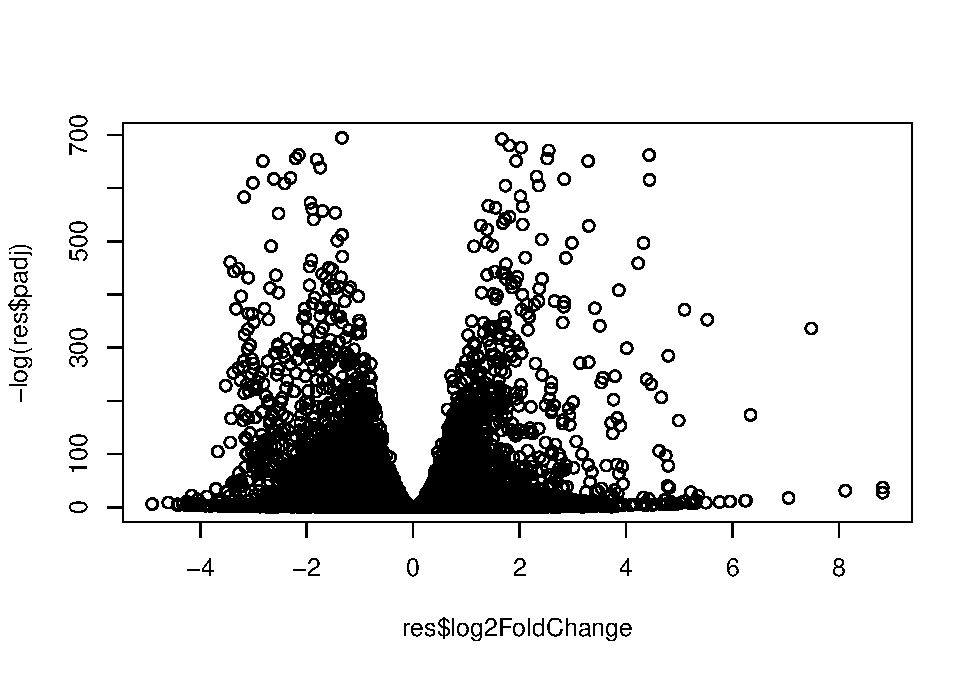
\includegraphics{lab13_bimm143_files/figure-latex/unnamed-chunk-9-1.pdf}

\begin{quote}
Q. Improve this plot by completing the below code, which adds color and
axis labels
\end{quote}

\begin{Shaded}
\begin{Highlighting}[]
\CommentTok{\# Make a color vector for all genes}
\NormalTok{mycols }\OtherTok{\textless{}{-}} \FunctionTok{rep}\NormalTok{(}\StringTok{"gray"}\NormalTok{, }\FunctionTok{nrow}\NormalTok{(res) )}

\CommentTok{\# Color red the genes with absolute fold change above 2}
\NormalTok{mycols[ }\FunctionTok{abs}\NormalTok{(res}\SpecialCharTok{$}\NormalTok{log2FoldChange) }\SpecialCharTok{\textgreater{}} \DecValTok{2}\NormalTok{ ] }\OtherTok{\textless{}{-}} \StringTok{"red"}

\CommentTok{\# Color blue those with adjusted p{-}value less than 0.01}
\CommentTok{\#  and absolute fold change more than 2}
\NormalTok{inds }\OtherTok{\textless{}{-}}\NormalTok{ (res}\SpecialCharTok{$}\NormalTok{padj }\SpecialCharTok{\textless{}} \FloatTok{0.01}\NormalTok{) }\SpecialCharTok{\&}\NormalTok{ (}\FunctionTok{abs}\NormalTok{(res}\SpecialCharTok{$}\NormalTok{log2FoldChange) }\SpecialCharTok{\textgreater{}} \DecValTok{2}\NormalTok{ )}
\NormalTok{mycols[ inds ] }\OtherTok{\textless{}{-}} \StringTok{"blue"}

\FunctionTok{plot}\NormalTok{( res}\SpecialCharTok{$}\NormalTok{log2FoldChange, }\SpecialCharTok{{-}}\FunctionTok{log}\NormalTok{(res}\SpecialCharTok{$}\NormalTok{padj), }\AttributeTok{col=}\NormalTok{mycols, }\AttributeTok{xlab=}\StringTok{"Log2(FoldChange)"}\NormalTok{, }\AttributeTok{ylab=}\StringTok{"{-}Log(P{-}value)"}\NormalTok{) }
\end{Highlighting}
\end{Shaded}

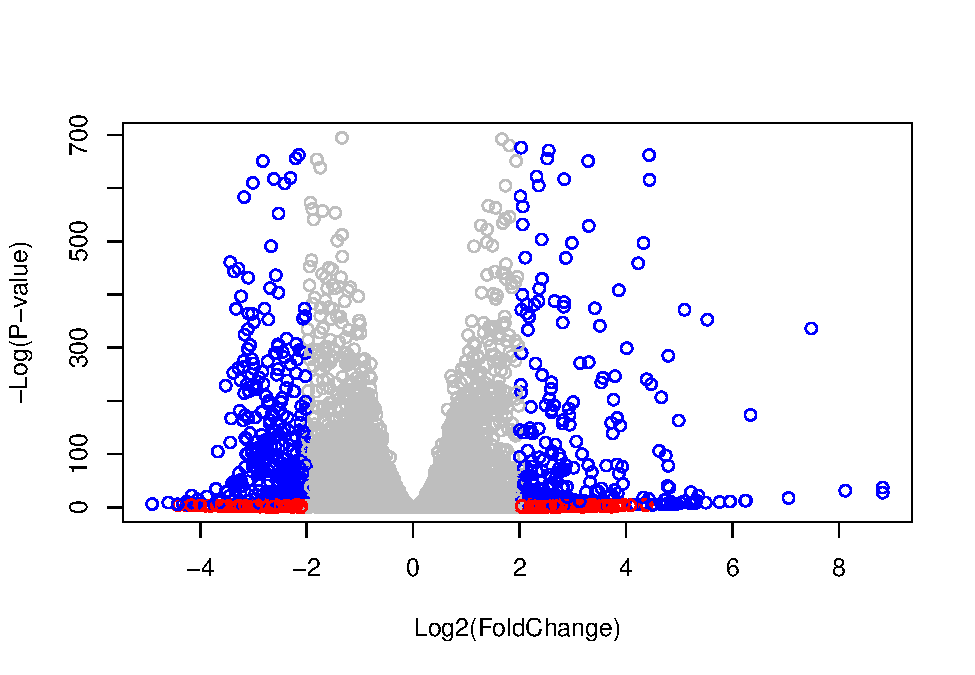
\includegraphics{lab13_bimm143_files/figure-latex/unnamed-chunk-10-1.pdf}

\hypertarget{annotate-results}{%
\subsection{Annotate Results}\label{annotate-results}}

\begin{Shaded}
\begin{Highlighting}[]
\FunctionTok{library}\NormalTok{(}\StringTok{"AnnotationDbi"}\NormalTok{)}
\end{Highlighting}
\end{Shaded}

\begin{Shaded}
\begin{Highlighting}[]
\FunctionTok{library}\NormalTok{(}\StringTok{"org.Hs.eg.db"}\NormalTok{)}
\end{Highlighting}
\end{Shaded}

\begin{verbatim}
## 
\end{verbatim}

\begin{quote}
\textbf{Q}. Use the~\textbf{mapIDs()}~function multiple times to add
SYMBOL, ENTREZID and GENENAME annotation to our results by completing
the code below.
\end{quote}

\begin{Shaded}
\begin{Highlighting}[]
\FunctionTok{columns}\NormalTok{(org.Hs.eg.db)}
\end{Highlighting}
\end{Shaded}

\begin{verbatim}
##  [1] "ACCNUM"       "ALIAS"        "ENSEMBL"      "ENSEMBLPROT"  "ENSEMBLTRANS"
##  [6] "ENTREZID"     "ENZYME"       "EVIDENCE"     "EVIDENCEALL"  "GENENAME"    
## [11] "GENETYPE"     "GO"           "GOALL"        "IPI"          "MAP"         
## [16] "OMIM"         "ONTOLOGY"     "ONTOLOGYALL"  "PATH"         "PFAM"        
## [21] "PMID"         "PROSITE"      "REFSEQ"       "SYMBOL"       "UCSCKG"      
## [26] "UNIPROT"
\end{verbatim}

\begin{Shaded}
\begin{Highlighting}[]
\NormalTok{res}\SpecialCharTok{$}\NormalTok{symbol }\OtherTok{=} \FunctionTok{mapIds}\NormalTok{(org.Hs.eg.db,}
                    \AttributeTok{keys=}\FunctionTok{row.names}\NormalTok{(res), }
                    \AttributeTok{keytype=}\StringTok{"ENSEMBL"}\NormalTok{,}
                    \AttributeTok{column=}\StringTok{"SYMBOL"}\NormalTok{,}
                    \AttributeTok{multiVals=}\StringTok{"first"}\NormalTok{)}
\end{Highlighting}
\end{Shaded}

\begin{verbatim}
## 'select()' returned 1:many mapping between keys and columns
\end{verbatim}

\begin{Shaded}
\begin{Highlighting}[]
\NormalTok{res}\SpecialCharTok{$}\NormalTok{entrez }\OtherTok{=} \FunctionTok{mapIds}\NormalTok{(org.Hs.eg.db,}
                    \AttributeTok{keys=}\FunctionTok{row.names}\NormalTok{(res),}
                    \AttributeTok{keytype=}\StringTok{"ENSEMBL"}\NormalTok{,}
                    \AttributeTok{column=}\StringTok{"ENTREZID"}\NormalTok{,}
                    \AttributeTok{multiVals=}\StringTok{"first"}\NormalTok{)}
\end{Highlighting}
\end{Shaded}

\begin{verbatim}
## 'select()' returned 1:many mapping between keys and columns
\end{verbatim}

\begin{Shaded}
\begin{Highlighting}[]
\NormalTok{res}\SpecialCharTok{$}\NormalTok{name }\OtherTok{=}   \FunctionTok{mapIds}\NormalTok{(org.Hs.eg.db,}
                    \AttributeTok{keys=}\FunctionTok{row.names}\NormalTok{(res),}
                    \AttributeTok{keytype=}\StringTok{"ENSEMBL"}\NormalTok{,}
                    \AttributeTok{column=}\StringTok{"GENENAME"}\NormalTok{,}
                    \AttributeTok{multiVals=}\StringTok{"first"}\NormalTok{)}
\end{Highlighting}
\end{Shaded}

\begin{verbatim}
## 'select()' returned 1:many mapping between keys and columns
\end{verbatim}

\begin{Shaded}
\begin{Highlighting}[]
\FunctionTok{head}\NormalTok{(res, }\DecValTok{10}\NormalTok{)}
\end{Highlighting}
\end{Shaded}

\begin{verbatim}
## log2 fold change (MLE): condition hoxa1_kd vs control_sirna 
## Wald test p-value: condition hoxa1 kd vs control sirna 
## DataFrame with 10 rows and 9 columns
##                    baseMean log2FoldChange     lfcSE       stat      pvalue
##                   <numeric>      <numeric> <numeric>  <numeric>   <numeric>
## ENSG00000279457   29.913579      0.1792571 0.3248216   0.551863 5.81042e-01
## ENSG00000187634  183.229650      0.4264571 0.1402658   3.040350 2.36304e-03
## ENSG00000188976 1651.188076     -0.6927205 0.0548465 -12.630158 1.43990e-36
## ENSG00000187961  209.637938      0.7297556 0.1318599   5.534326 3.12428e-08
## ENSG00000187583   47.255123      0.0405765 0.2718928   0.149237 8.81366e-01
## ENSG00000187642   11.979750      0.5428105 0.5215598   1.040744 2.97994e-01
## ENSG00000188290  108.922128      2.0570638 0.1969053  10.446970 1.51282e-25
## ENSG00000187608  350.716868      0.2573837 0.1027266   2.505522 1.22271e-02
## ENSG00000188157 9128.439422      0.3899088 0.0467163   8.346304 7.04321e-17
## ENSG00000237330    0.158192      0.7859552 4.0804729   0.192614 8.47261e-01
##                        padj      symbol      entrez                   name
##                   <numeric> <character> <character>            <character>
## ENSG00000279457 6.86555e-01          NA          NA                     NA
## ENSG00000187634 5.15718e-03      SAMD11      148398 sterile alpha motif ..
## ENSG00000188976 1.76549e-35       NOC2L       26155 NOC2 like nucleolar ..
## ENSG00000187961 1.13413e-07      KLHL17      339451 kelch like family me..
## ENSG00000187583 9.19031e-01     PLEKHN1       84069 pleckstrin homology ..
## ENSG00000187642 4.03379e-01       PERM1       84808 PPARGC1 and ESRR ind..
## ENSG00000188290 1.30538e-24        HES4       57801 hes family bHLH tran..
## ENSG00000187608 2.37452e-02       ISG15        9636 ISG15 ubiquitin like..
## ENSG00000188157 4.21963e-16        AGRN      375790                  agrin
## ENSG00000237330          NA      RNF223      401934 ring finger protein ..
\end{verbatim}

\hypertarget{save-results}{%
\subsection{Save results}\label{save-results}}

\begin{Shaded}
\begin{Highlighting}[]
\NormalTok{res }\OtherTok{=}\NormalTok{ res[}\FunctionTok{order}\NormalTok{(res}\SpecialCharTok{$}\NormalTok{pvalue),]}
\FunctionTok{write.csv}\NormalTok{(res, }\AttributeTok{file =} \StringTok{"myresults.csv"}\NormalTok{)}
\end{Highlighting}
\end{Shaded}

\hypertarget{pathway-analysis}{%
\subsection{Pathway Analysis}\label{pathway-analysis}}

\begin{Shaded}
\begin{Highlighting}[]
\FunctionTok{library}\NormalTok{(pathview)}
\end{Highlighting}
\end{Shaded}

\begin{verbatim}
## ##############################################################################
## Pathview is an open source software package distributed under GNU General
## Public License version 3 (GPLv3). Details of GPLv3 is available at
## http://www.gnu.org/licenses/gpl-3.0.html. Particullary, users are required to
## formally cite the original Pathview paper (not just mention it) in publications
## or products. For details, do citation("pathview") within R.
## 
## The pathview downloads and uses KEGG data. Non-academic uses may require a KEGG
## license agreement (details at http://www.kegg.jp/kegg/legal.html).
## ##############################################################################
\end{verbatim}

\begin{Shaded}
\begin{Highlighting}[]
\FunctionTok{library}\NormalTok{(gage)}
\end{Highlighting}
\end{Shaded}

\begin{verbatim}
## 
\end{verbatim}

\begin{Shaded}
\begin{Highlighting}[]
\FunctionTok{library}\NormalTok{(gageData)}
\end{Highlighting}
\end{Shaded}

\begin{Shaded}
\begin{Highlighting}[]
\FunctionTok{data}\NormalTok{(kegg.sets.hs)}
\FunctionTok{data}\NormalTok{(sigmet.idx.hs)}

\NormalTok{kegg.sets.hs }\OtherTok{=}\NormalTok{ kegg.sets.hs[sigmet.idx.hs]}

\FunctionTok{head}\NormalTok{(kegg.sets.hs, }\DecValTok{3}\NormalTok{)}
\end{Highlighting}
\end{Shaded}

\begin{verbatim}
## $`hsa00232 Caffeine metabolism`
## [1] "10"   "1544" "1548" "1549" "1553" "7498" "9"   
## 
## $`hsa00983 Drug metabolism - other enzymes`
##  [1] "10"     "1066"   "10720"  "10941"  "151531" "1548"   "1549"   "1551"  
##  [9] "1553"   "1576"   "1577"   "1806"   "1807"   "1890"   "221223" "2990"  
## [17] "3251"   "3614"   "3615"   "3704"   "51733"  "54490"  "54575"  "54576" 
## [25] "54577"  "54578"  "54579"  "54600"  "54657"  "54658"  "54659"  "54963" 
## [33] "574537" "64816"  "7083"   "7084"   "7172"   "7363"   "7364"   "7365"  
## [41] "7366"   "7367"   "7371"   "7372"   "7378"   "7498"   "79799"  "83549" 
## [49] "8824"   "8833"   "9"      "978"   
## 
## $`hsa00230 Purine metabolism`
##   [1] "100"    "10201"  "10606"  "10621"  "10622"  "10623"  "107"    "10714" 
##   [9] "108"    "10846"  "109"    "111"    "11128"  "11164"  "112"    "113"   
##  [17] "114"    "115"    "122481" "122622" "124583" "132"    "158"    "159"   
##  [25] "1633"   "171568" "1716"   "196883" "203"    "204"    "205"    "221823"
##  [33] "2272"   "22978"  "23649"  "246721" "25885"  "2618"   "26289"  "270"   
##  [41] "271"    "27115"  "272"    "2766"   "2977"   "2982"   "2983"   "2984"  
##  [49] "2986"   "2987"   "29922"  "3000"   "30833"  "30834"  "318"    "3251"  
##  [57] "353"    "3614"   "3615"   "3704"   "377841" "471"    "4830"   "4831"  
##  [65] "4832"   "4833"   "4860"   "4881"   "4882"   "4907"   "50484"  "50940" 
##  [73] "51082"  "51251"  "51292"  "5136"   "5137"   "5138"   "5139"   "5140"  
##  [81] "5141"   "5142"   "5143"   "5144"   "5145"   "5146"   "5147"   "5148"  
##  [89] "5149"   "5150"   "5151"   "5152"   "5153"   "5158"   "5167"   "5169"  
##  [97] "51728"  "5198"   "5236"   "5313"   "5315"   "53343"  "54107"  "5422"  
## [105] "5424"   "5425"   "5426"   "5427"   "5430"   "5431"   "5432"   "5433"  
## [113] "5434"   "5435"   "5436"   "5437"   "5438"   "5439"   "5440"   "5441"  
## [121] "5471"   "548644" "55276"  "5557"   "5558"   "55703"  "55811"  "55821" 
## [129] "5631"   "5634"   "56655"  "56953"  "56985"  "57804"  "58497"  "6240"  
## [137] "6241"   "64425"  "646625" "654364" "661"    "7498"   "8382"   "84172" 
## [145] "84265"  "84284"  "84618"  "8622"   "8654"   "87178"  "8833"   "9060"  
## [153] "9061"   "93034"  "953"    "9533"   "954"    "955"    "956"    "957"   
## [161] "9583"   "9615"
\end{verbatim}

\begin{Shaded}
\begin{Highlighting}[]
\NormalTok{foldchanges }\OtherTok{=}\NormalTok{ res}\SpecialCharTok{$}\NormalTok{log2FoldChange}

\FunctionTok{names}\NormalTok{(foldchanges) }\OtherTok{=}\NormalTok{ res}\SpecialCharTok{$}\NormalTok{entrez}
\FunctionTok{head}\NormalTok{(foldchanges)}
\end{Highlighting}
\end{Shaded}

\begin{verbatim}
##      1266     54855      1465     51232      2034      2317 
## -2.422719  3.201955 -2.313738 -2.059631 -1.888019 -1.649792
\end{verbatim}

\begin{Shaded}
\begin{Highlighting}[]
\NormalTok{keggres }\OtherTok{=} \FunctionTok{gage}\NormalTok{(foldchanges, }\AttributeTok{gsets =}\NormalTok{ kegg.sets.hs)}
\end{Highlighting}
\end{Shaded}

\begin{Shaded}
\begin{Highlighting}[]
\FunctionTok{attributes}\NormalTok{(keggres)}
\end{Highlighting}
\end{Shaded}

\begin{verbatim}
## $names
## [1] "greater" "less"    "stats"
\end{verbatim}

\begin{Shaded}
\begin{Highlighting}[]
\FunctionTok{head}\NormalTok{(keggres}\SpecialCharTok{$}\NormalTok{less)}
\end{Highlighting}
\end{Shaded}

\begin{verbatim}
##                                          p.geomean stat.mean        p.val
## hsa04110 Cell cycle                   8.995727e-06 -4.378644 8.995727e-06
## hsa03030 DNA replication              9.424076e-05 -3.951803 9.424076e-05
## hsa03013 RNA transport                1.375901e-03 -3.028500 1.375901e-03
## hsa03440 Homologous recombination     3.066756e-03 -2.852899 3.066756e-03
## hsa04114 Oocyte meiosis               3.784520e-03 -2.698128 3.784520e-03
## hsa00010 Glycolysis / Gluconeogenesis 8.961413e-03 -2.405398 8.961413e-03
##                                             q.val set.size         exp1
## hsa04110 Cell cycle                   0.001448312      121 8.995727e-06
## hsa03030 DNA replication              0.007586381       36 9.424076e-05
## hsa03013 RNA transport                0.073840037      144 1.375901e-03
## hsa03440 Homologous recombination     0.121861535       28 3.066756e-03
## hsa04114 Oocyte meiosis               0.121861535      102 3.784520e-03
## hsa00010 Glycolysis / Gluconeogenesis 0.212222694       53 8.961413e-03
\end{verbatim}

\begin{Shaded}
\begin{Highlighting}[]
\FunctionTok{pathview}\NormalTok{(}\AttributeTok{gene.data=}\NormalTok{foldchanges, }\AttributeTok{pathway.id=}\StringTok{"hsa04110"}\NormalTok{)}
\end{Highlighting}
\end{Shaded}

\begin{verbatim}
## 'select()' returned 1:1 mapping between keys and columns
\end{verbatim}

\begin{verbatim}
## Info: Working in directory C:/Users/AJCag/OneDrive/Desktop/Lab 13
\end{verbatim}

\begin{verbatim}
## Info: Writing image file hsa04110.pathview.png
\end{verbatim}

\begin{figure}
\centering
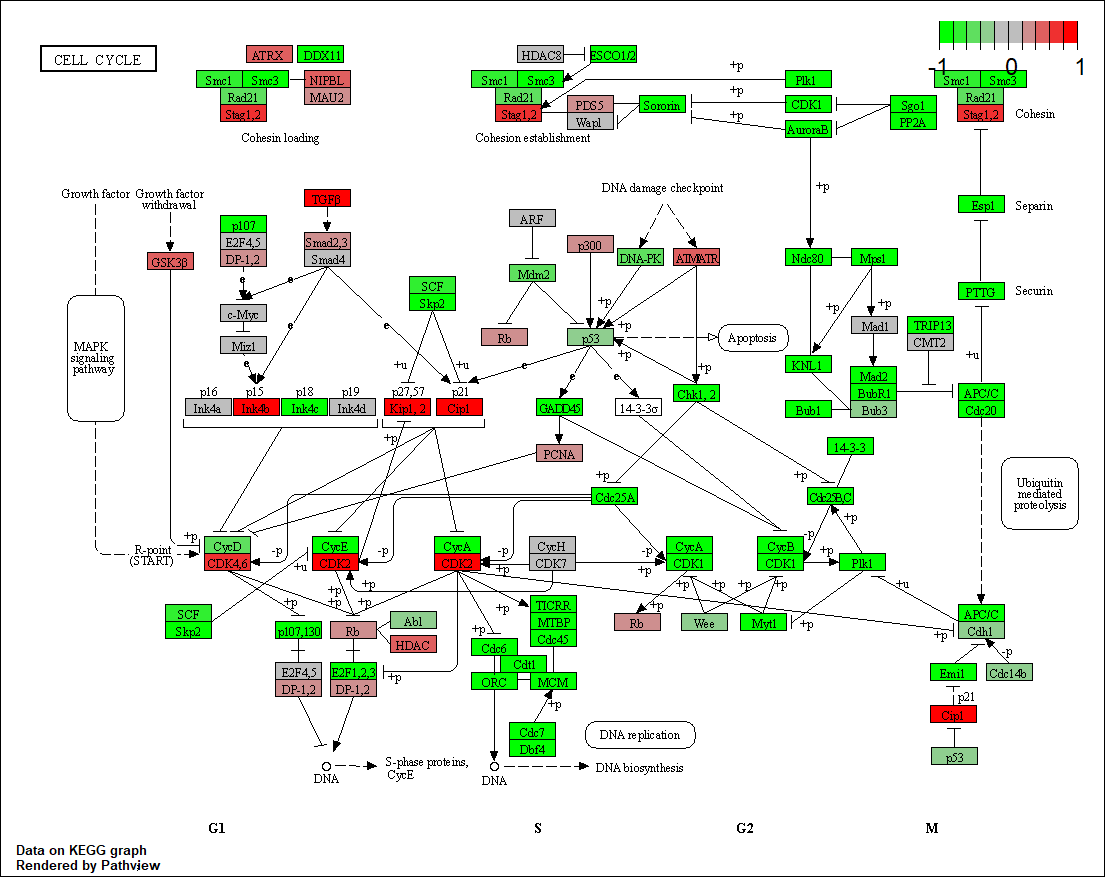
\includegraphics{hsa04110.pathview.png}
\caption{Pathway analysis}
\end{figure}

\begin{Shaded}
\begin{Highlighting}[]
\CommentTok{\# A different PDF based output of the same data}
\FunctionTok{pathview}\NormalTok{(}\AttributeTok{gene.data=}\NormalTok{foldchanges, }\AttributeTok{pathway.id=}\StringTok{"hsa04110"}\NormalTok{, }\AttributeTok{kegg.native=}\ConstantTok{FALSE}\NormalTok{)}
\end{Highlighting}
\end{Shaded}

\begin{verbatim}
## 'select()' returned 1:1 mapping between keys and columns
\end{verbatim}

\begin{verbatim}
## Warning: reconcile groups sharing member nodes!
\end{verbatim}

\begin{verbatim}
##      [,1] [,2] 
## [1,] "9"  "300"
## [2,] "9"  "306"
\end{verbatim}

\begin{verbatim}
## Info: Working in directory C:/Users/AJCag/OneDrive/Desktop/Lab 13
\end{verbatim}

\begin{verbatim}
## Info: Writing image file hsa04110.pathview.pdf
\end{verbatim}

\begin{Shaded}
\begin{Highlighting}[]
\DocumentationTok{\#\# Focus on top 5 upregulated pathways here for demo purposes only}
\NormalTok{keggrespathways }\OtherTok{\textless{}{-}} \FunctionTok{rownames}\NormalTok{(keggres}\SpecialCharTok{$}\NormalTok{greater)[}\DecValTok{1}\SpecialCharTok{:}\DecValTok{5}\NormalTok{]}

\CommentTok{\# Extract the 8 character long IDs part of each string}
\NormalTok{keggresids }\OtherTok{=} \FunctionTok{substr}\NormalTok{(keggrespathways, }\AttributeTok{start=}\DecValTok{1}\NormalTok{, }\AttributeTok{stop=}\DecValTok{8}\NormalTok{)}
\NormalTok{keggresids}
\end{Highlighting}
\end{Shaded}

\begin{verbatim}
## [1] "hsa04640" "hsa04630" "hsa00140" "hsa04142" "hsa04330"
\end{verbatim}

\begin{Shaded}
\begin{Highlighting}[]
\NormalTok{sig\_genes }\OtherTok{\textless{}{-}}\NormalTok{ res[res}\SpecialCharTok{$}\NormalTok{padj }\SpecialCharTok{\textless{}=} \FloatTok{0.05} \SpecialCharTok{\&} \SpecialCharTok{!}\FunctionTok{is.na}\NormalTok{(res}\SpecialCharTok{$}\NormalTok{padj), }\StringTok{"symbol"}\NormalTok{]}
\FunctionTok{print}\NormalTok{(}\FunctionTok{paste}\NormalTok{(}\StringTok{"Total number of significant genes:"}\NormalTok{, }\FunctionTok{length}\NormalTok{(sig\_genes)))}
\end{Highlighting}
\end{Shaded}

\begin{verbatim}
## [1] "Total number of significant genes: 8147"
\end{verbatim}

\begin{Shaded}
\begin{Highlighting}[]
\FunctionTok{write.table}\NormalTok{(sig\_genes, }\AttributeTok{file=}\StringTok{"significant\_genes.txt"}\NormalTok{, }\AttributeTok{row.names=}\ConstantTok{FALSE}\NormalTok{, }\AttributeTok{col.names=}\ConstantTok{FALSE}\NormalTok{, }\AttributeTok{quote=}\ConstantTok{FALSE}\NormalTok{)}
\end{Highlighting}
\end{Shaded}

\hypertarget{gene-ontology}{%
\subsection{Gene Ontology}\label{gene-ontology}}

\begin{Shaded}
\begin{Highlighting}[]
\CommentTok{\#data(go.sets.hs)}
\CommentTok{\#data(go.subs.hs)}

\CommentTok{\# Focus on Biological Process subset of GO}
\CommentTok{\#gobpsets = go.sets.hs[go.subs.hs$BP]}

\CommentTok{\#gobpres = gage(foldchanges, gsets=gobpsets, same.dir=TRUE)}

\CommentTok{\#lapply(gobpres, head)}
\end{Highlighting}
\end{Shaded}

\hypertarget{reactome-analysis}{%
\subsection{Reactome Analysis}\label{reactome-analysis}}

\begin{Shaded}
\begin{Highlighting}[]
\NormalTok{sig\_genes }\OtherTok{\textless{}{-}}\NormalTok{ res[res}\SpecialCharTok{$}\NormalTok{padj }\SpecialCharTok{\textless{}=} \FloatTok{0.05} \SpecialCharTok{\&} \SpecialCharTok{!}\FunctionTok{is.na}\NormalTok{(res}\SpecialCharTok{$}\NormalTok{padj), }\StringTok{"symbol"}\NormalTok{]}
\FunctionTok{print}\NormalTok{(}\FunctionTok{paste}\NormalTok{(}\StringTok{"Total number of significant genes:"}\NormalTok{, }\FunctionTok{length}\NormalTok{(sig\_genes)))}
\end{Highlighting}
\end{Shaded}

\begin{verbatim}
## [1] "Total number of significant genes: 8147"
\end{verbatim}

\begin{Shaded}
\begin{Highlighting}[]
\FunctionTok{write.table}\NormalTok{(sig\_genes, }\AttributeTok{file=}\StringTok{"significant\_genes.txt"}\NormalTok{, }\AttributeTok{row.names=}\ConstantTok{FALSE}\NormalTok{, }\AttributeTok{col.names=}\ConstantTok{FALSE}\NormalTok{, }\AttributeTok{quote=}\ConstantTok{FALSE}\NormalTok{)}
\end{Highlighting}
\end{Shaded}


\end{document}
